\section{Implementation} \label{sec:implementation}

\subsection{Parameters of the Implementation}


\begin{table}[tbh]
\begin{center}
\begin{tabular}{p{.2 \textwidth} | p{.6 \textwidth} | p{.2 \textwidth}}\hline
Field & Description & Default value\\ \hline
$P\in\mathbb{Z}$ & Number of populations. & 1 \\
$n\in\mathbb{Z}$ & Maximum number of pure strategies per population. & - \\
$S\in\mathbb{Z}^{P}$ & Vector of pure strategies in each population, such that $1<S(i)\leq n$. & ones(G.P, 1) * G.n \\
$m\in\mathbb{R}^P$ & Vector with the mass of each population. & ones(G.P, 1) \\
$x0\in\mathbb{R}^{P\times n}$ & Initial state of the society (normalized). & random \\
$f:\mathbb{R}^{P\times n} \rightarrow \mathbb{R}^{1\times n}$ or $f:\mathbb{R}^{P\times n} \rightarrow \mathbb{R}^{P\times n}$ & Function that returns the fitness the population's strategies. It might return a vector with the fitness of a single population or the fitness of the whole society. & - \\ 
pop\_wise & If true, the fitness function $f$ returns the fitness of a single population. Otherwise, $f$ returns the fitness of the whole society. & True \\
\hline
\end{tabular}
\end{center}
\caption{Parameters of the game.}
\label{tab:game}
\end{table}



\begin{table}[tbh]
\begin{center}
\begin{tabular}{p{.2 \textwidth} | p{.6 \textwidth} | p{.2 \textwidth}}\hline
Field & Description & Default value\\ \hline
ode & ODE solver for the evolutionary dynamics. & `ode45' \\
dynamics & Evolutionary dynamic. Current version support combinations of {`rd', `maynard\_rd',  `bnn', `smith',  `logit'}. & `rd' \\
gamma & Defines the weight given to each dynamic when using combined dynamics. &  $\sum \gamma(i) = 1$ \\
step & Simulations are made using the time spam: step:step:time+step. & $0.01$ \\
tol & Defines the error tolerance of the ODE solver, namely, RelTol and AbsTol. If it is not defined, then RelTol and AbsTol can be assigned independently. &  RelTol=AbsTol=$10^{-4}$\\
stop\_c  & Enables the interruption of the simulations if the norm of the state's change is less than the parameter c\_error. & False \\
c\_error &  Convergence error used to stop the simulations. & $10^{-5}$ \\
verb & Allows the display of information, such as the dynamics used and the time spent running the game. & True \\
\hline
\end{tabular}
\end{center}
\caption{Parameters of the dynamical implementation.}
\label{tab:req_a}
\end{table}




\begin{table}[tbh]
\begin{center}
\begin{tabular}{p{.2 \textwidth} | p{.6 \textwidth} | p{.2 \textwidth}}\hline
Field & Description & Default value \\ \hline
$N\in\mathbb{Z}$ & Number of agents & 100 \\
$R\in\mathbb{R}$ & Rate of the Poisson clock & 1 \\
time & Run time of the simulation (number of iterations in the discrete case). & 30 \\
revision\_protocol & Revision protocol. The current version support one of the following: `comparison2average', `pairwise\_comparison', `logit\_choice', `proportional\_imitation'. & `proportional\_imitation' \\ \hline
\end{tabular}
\end{center}
\caption{Parameters of the revision protocol.}
\label{tab:req_b}
\end{table}




The toolbox uses a structure that contains all the parameters required to run the simulations. The parameters of a population game are defined in Table \ref{tab:game}. On the other hand, the parameters to run simulations with large or small number of agents are specified in Tables \ref{tab:req_a} and \ref{tab:req_b}, respectively.  In this case the behavior of a population with large and small number of agents is simulated using differential equations and revision protocols, respectively. The following is an example to define a game with one population and three strategies per population:
%
\begin{lstlisting}
G = struct('n', 3, 'f', @fitness1, 'dynamics', {rd},  'ode', 'ode113', 'x0',  [0.2 .7 0.1]', 'time', 60);
\end{lstlisting}
%
$n$ defines the number of strategies per population, $f$ is a function handler that calculates the fitness of the strategies in each population, and $dynamics$ defines the name of the evolutionary dynamics that we want to use. The simulations are run using the ordinal differential equation (ODE) solver called $ode113$, with initial condition $x0 = [0.2, \, 0.7, \, 0.1 ]^\top$ during $60$ time units.
Note that the number of populations and the mass of each population are defined by default to one.  The simulation can be started by executing
%
\begin{lstlisting}
 G.run()
\end{lstlisting}




On the other hand, the following structure is used to define a population game with small number of agents per population:
%
\begin{lstlisting}
G = struct('N', 200, 'n', 3, 'f', @fitness1, 'x0',  [0.2 .7 0.1]', 'ode', 'ode113', 'time', 10000, 'eta', 0.02, 'revision_protocol', @proportional_imitation); 
\end{lstlisting}
%
The finite population case uses the same parameters than the dynamical implementation, except for the dynamical model. However, it is necessary to define the revision protocol  and the number of agents $N$ per population.
Table \ref{tab:req_b} contains the list of parameters required to run the revision protocol. The simulation of the revision protocol can be started by executing
\begin{lstlisting}
 G.run_finite()
\end{lstlisting}

The functions \verb|G.graph()| and \verb|G.graph_evolution()| can be used to graph the simplex and the state evolution of the society for both cases.



\subsection{Example: Rock-Paper-Scissors Game}



\begin{figure}[th]
  \centering
  \begin{subfigure}[b]{0.4\textwidth}
	  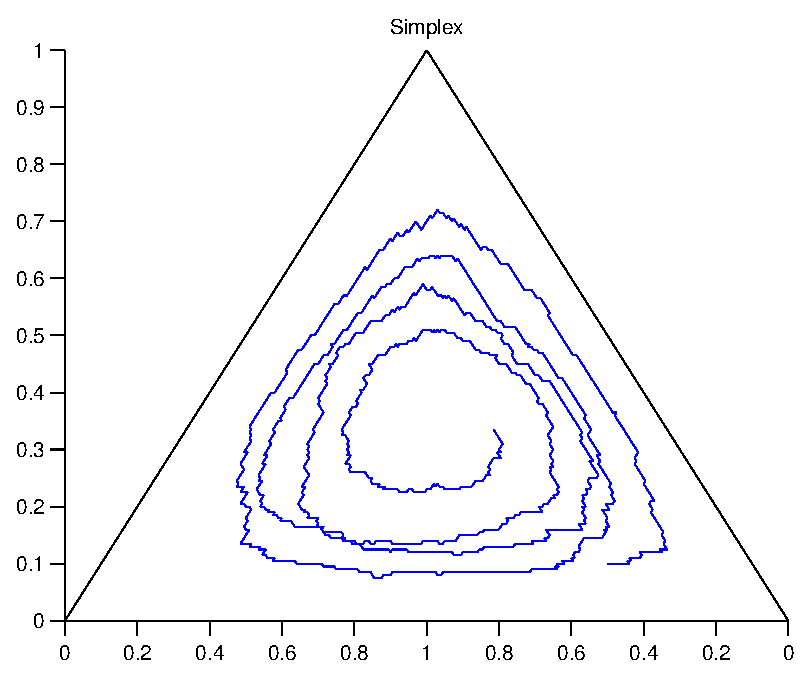
\includegraphics[width=\textwidth]{./images/test_finite_proportional_imitation.eps}
	  \caption{Small population.}
	  \label{fig:finite1_protocol}
  \end{subfigure}
  ~ 
  \begin{subfigure}[b]{0.4\textwidth}
	  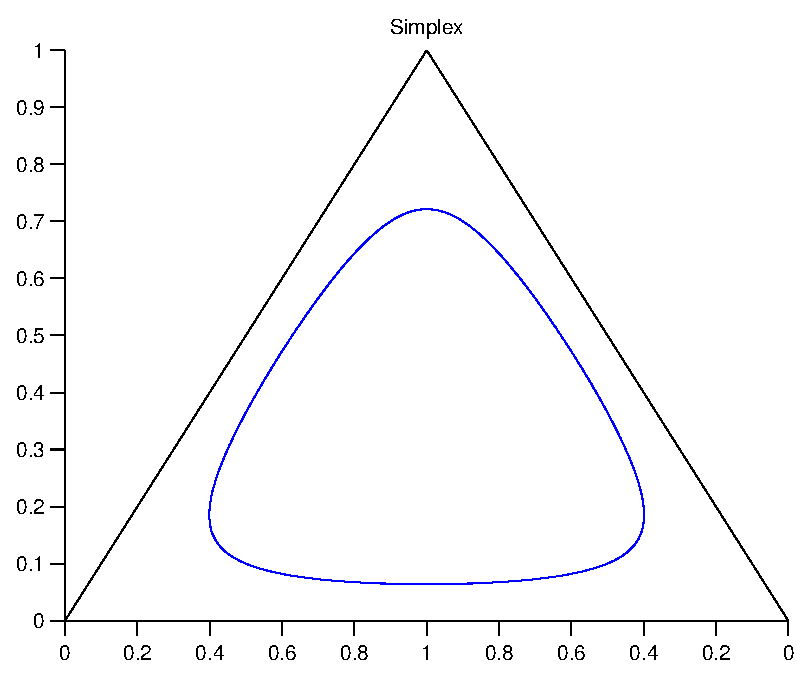
\includegraphics[width=\textwidth]{./images/test1_simplex_rd.eps}
	  \caption{Large popultion.}
	  \label{fig:finite1_dynamics}
  \end{subfigure}
  \caption{Rock-paper-scissors game with a) proportional imitation revision protocol and b) replicator dynamics.}
  \label{fig:finite1}
\end{figure}


\begin{figure}[th]
  \centering
  \begin{subfigure}[b]{0.4\textwidth}
	  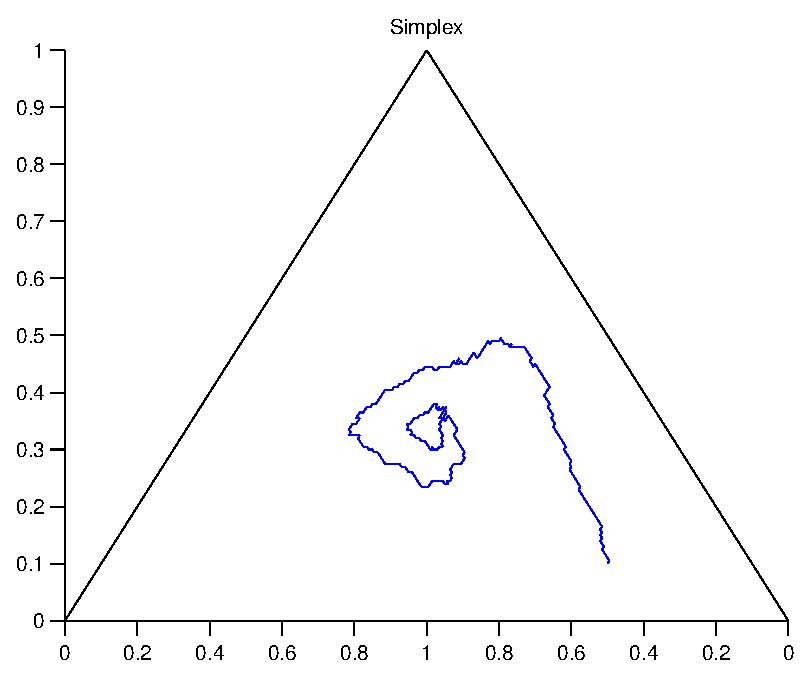
\includegraphics[width=\textwidth]{./images/test_finite_comparison2average.eps}
	  \caption{Small population.}
	  \label{fig:finite2_protocol}
  \end{subfigure}
  ~ 
  \begin{subfigure}[b]{0.4\textwidth}
	  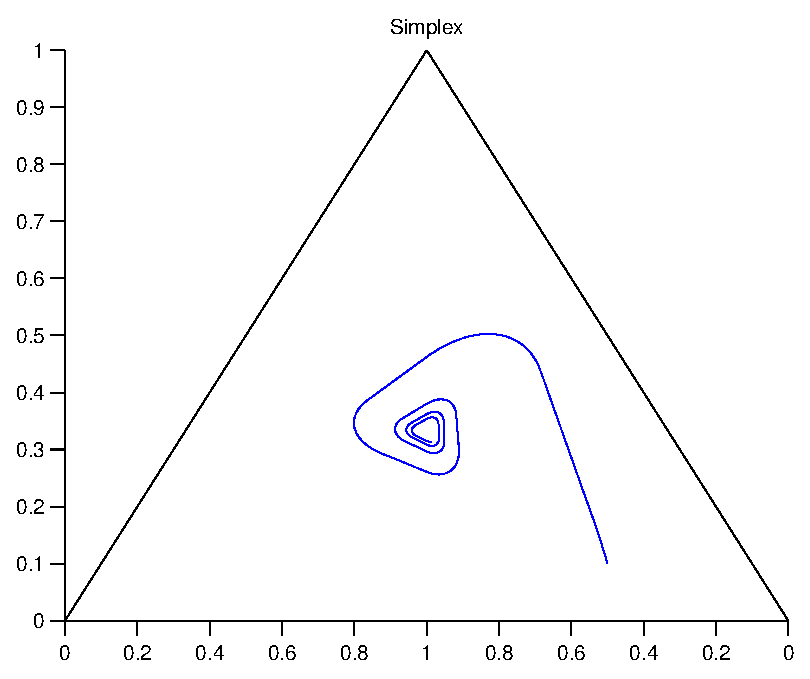
\includegraphics[width=\textwidth]{./images/test1_simplex_bnn.eps}
	  \caption{Large popultion.}
	  \label{fig:finite2_dynamics}
  \end{subfigure}
  \caption{Rock-paper-scissors game with a) comparison to average revision protocol and b) BNN dynamics.}
  \label{fig:finite2}
\end{figure}


\begin{figure}[tbh]
  \centering
  \begin{subfigure}[b]{0.4\textwidth}
	  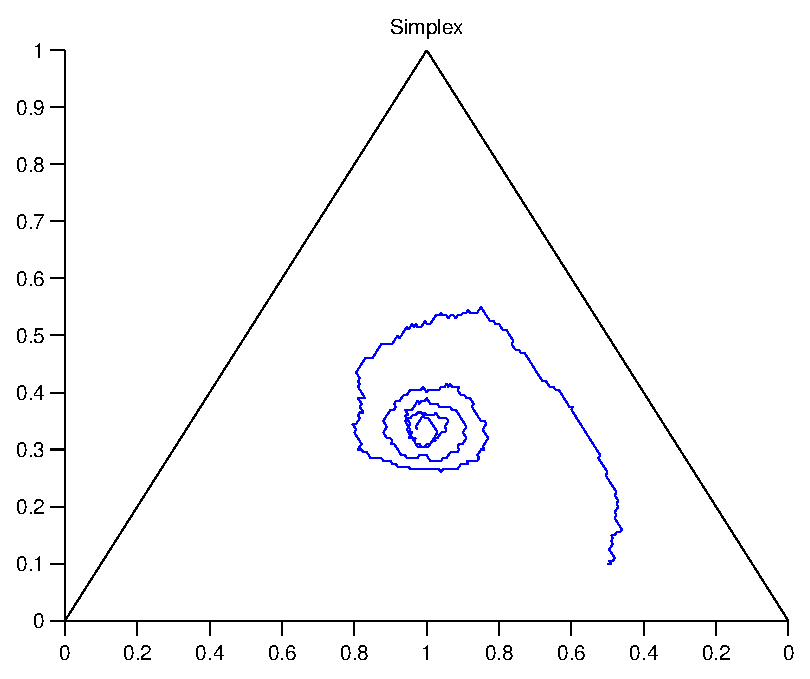
\includegraphics[width=\textwidth]{./images/test_finite_pairwise_comparison.eps}
	  \caption{Small population.}
	  \label{fig:finite3_protocol}
  \end{subfigure}
  ~ 
  \begin{subfigure}[b]{0.4\textwidth}
	  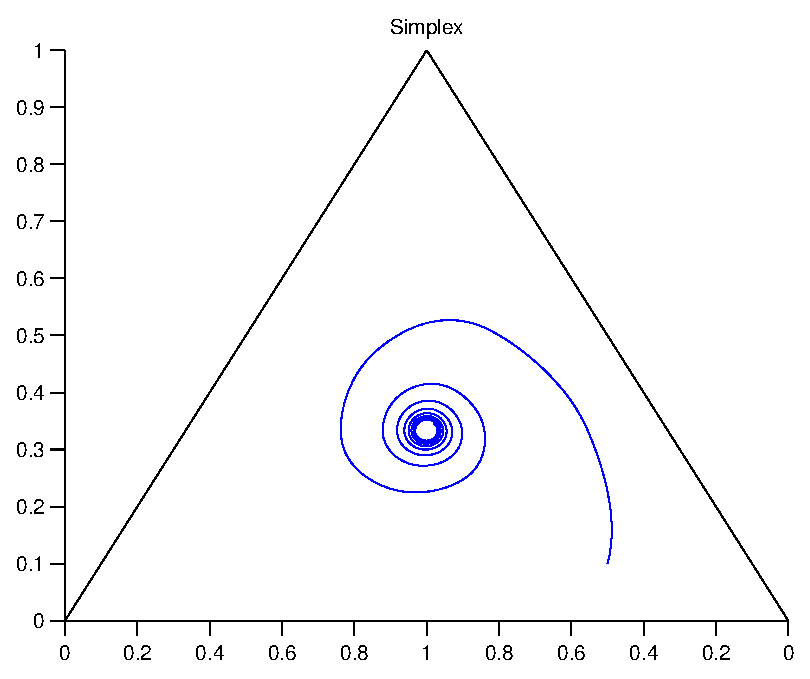
\includegraphics[width=\textwidth]{./images/test1_simplex_smith.eps}
	  \caption{Large popultion.}
	  \label{fig:finite3_dynamics}
  \end{subfigure}
  \caption{Rock-paper-scissors game with a) pairwise comparison revision protocol and b) Smith dynamics.}
  \label{fig:finite3}
\end{figure}


\begin{figure}[tbh]
  \centering
  \begin{subfigure}[b]{0.4\textwidth}
	  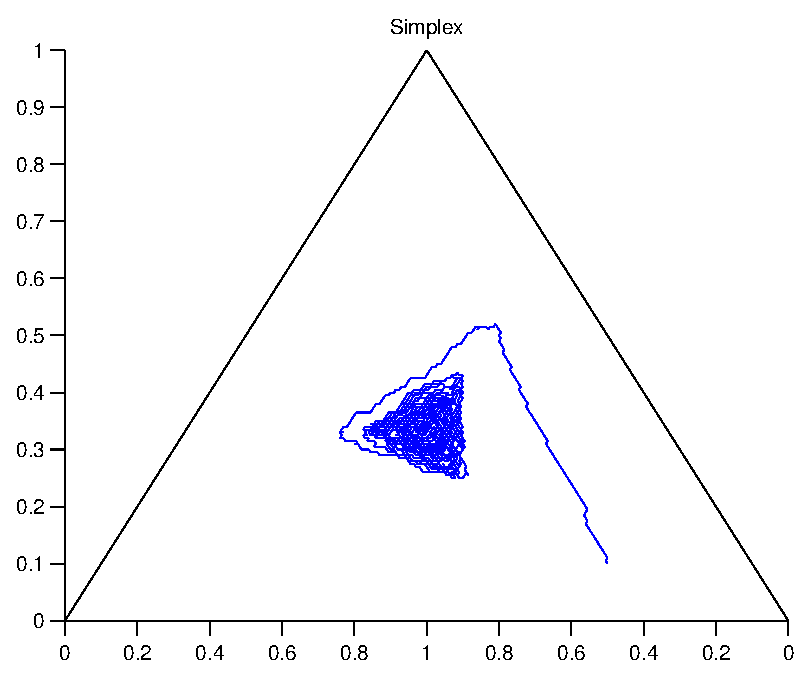
\includegraphics[width=\textwidth]{./images/test_finite_logit_choice.eps}
	  \caption{Small population.}
	  \label{fig:finite4_protocol}
  \end{subfigure}
  ~ 
  \begin{subfigure}[b]{0.4\textwidth}
	  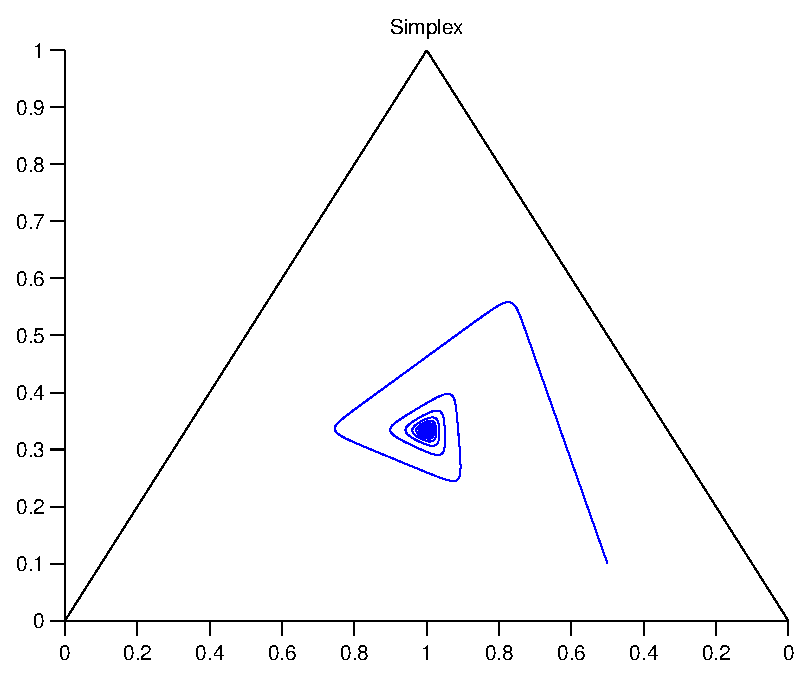
\includegraphics[width=\textwidth]{./images/test1_simplex_logit.eps}
	  \caption{Large popultion.}
	  \label{fig:finite4_dynamics}
  \end{subfigure}
  \caption{Rock-paper-scissors game with a) logit choice revision protocol and b) Logit dynamics with $\eta=0.02$.}
  \label{fig:finite4}
\end{figure}





In this section, we implement rock-paper-scissors game with both revision protocols and evolutionary dynamics presented above, to observe the behavioral differences between a society with small number of agents and its approximation to a dynamical system.
The game has only one population with three strategies, denoted $x = [x_1, \, x_2, \, x_3]^\top$. The fitness function is defined as $F(x)=Ax$, where A is equal to 
\begin{equation}
  A = \begin{pmatrix}
  2  & 1 &  3 \\
  3  & 2 &  1 \\
  1 &  3 &  2
  \end{pmatrix}
\end{equation}
Note that we modify the payoff matrix proposed in the literature to ensure positive payoffs.
Fig. \ref{fig:finite1} to \ref{fig:finite4} show the evolution of the society with each revision protocol and its approximation to differential equations. We set the initial condition $x_0 = [0.2, \, 0.7, \, 0.1 ]^\top$. The small population cases are made with $200$ agents and $10000$ iterations. The dynamical cases are run during 
30 time units.


%The evolution might take place in days, months, years.



